%%%%%%%%%%%%%%%%%%%%%%%%%%%%%%%%%%%%%%%%%
% Wenneker Article
% LaTeX Template
% Version 2.0 (28/2/17)
%
% This template was downloaded from:
% http://www.LaTeXTemplates.com
%
% Authors:
% Vel (vel@LaTeXTemplates.com)
% Frits Wenneker
%
% License:
% CC BY-NC-SA 3.0 (http://creativecommons.org/licenses/by-nc-sa/3.0/)
%
%%%%%%%%%%%%%%%%%%%%%%%%%%%%%%%%%%%%%%%%%

%----------------------------------------------------------------------------------------
%	PACKAGES AND OTHER DOCUMENT CONFIGURATIONS
%----------------------------------------------------------------------------------------

\documentclass[10pt, a4paper, twocolumn]{article} % 10pt font size (11 and 12 also possible), A4 paper (letterpaper for US letter) and two column layout (remove for one column)

%%%%%%%%%%%%%%%%%%%%%%%%%%%%%%%%%%%%%%%%%
% Wenneker Article
% Structure Specification File
% Version 1.0 (28/2/17)
%
% This file originates from:
% http://www.LaTeXTemplates.com
%
% Authors:
% Frits Wenneker
% Vel (vel@LaTeXTemplates.com)
%
% License:
% CC BY-NC-SA 3.0 (http://creativecommons.org/licenses/by-nc-sa/3.0/)
%
%%%%%%%%%%%%%%%%%%%%%%%%%%%%%%%%%%%%%%%%%

%----------------------------------------------------------------------------------------
%	PACKAGES AND OTHER DOCUMENT CONFIGURATIONS
%----------------------------------------------------------------------------------------

\usepackage[english]{babel} % English language hyphenation

\usepackage{microtype} % Better typography

\usepackage{amsmath,amsfonts,amsthm} % Math packages for equations

\usepackage[svgnames]{xcolor} % Enabling colors by their 'svgnames'

\usepackage[hang, small, labelfont=bf, up, textfont=it]{caption} % Custom captions under/above tables and figures

\usepackage{booktabs} % Horizontal rules in tables

\usepackage{lastpage} % Used to determine the number of pages in the document (for "Page X of Total")

\usepackage{graphicx} % Required for adding images

\usepackage{placeins} % For FloatBarrier

\usepackage{enumitem} % Required for customising lists
\setlist{noitemsep} % Remove spacing between bullet/numbered list elements

\usepackage{sectsty} % Enables custom section titles
\allsectionsfont{\usefont{OT1}{phv}{b}{n}} % Change the font of all section commands (Helvetica)

%----------------------------------------------------------------------------------------
%	MARGINS AND SPACING
%----------------------------------------------------------------------------------------

\usepackage{geometry} % Required for adjusting page dimensions

\geometry{
	top=1cm, % Top margin
	bottom=1.5cm, % Bottom margin
	left=2cm, % Left margin
	right=2cm, % Right margin
	includehead, % Include space for a header
	includefoot, % Include space for a footer
	%showframe, % Uncomment to show how the type block is set on the page
}

\setlength{\columnsep}{7mm} % Column separation width

%----------------------------------------------------------------------------------------
%	FONTS
%----------------------------------------------------------------------------------------

\usepackage[T1]{fontenc} % Output font encoding for international characters
\usepackage[utf8]{inputenc} % Required for inputting international characters

\usepackage{XCharter} % Use the XCharter font

%----------------------------------------------------------------------------------------
%	HEADERS AND FOOTERS
%----------------------------------------------------------------------------------------

\usepackage{fancyhdr} % Needed to define custom headers/footers
\pagestyle{fancy} % Enables the custom headers/footers

\renewcommand{\headrulewidth}{0.0pt} % No header rule
\renewcommand{\footrulewidth}{0.4pt} % Thin footer rule

\renewcommand{\sectionmark}[1]{\markboth{#1}{}} % Removes the section number from the header when \leftmark is used

%\nouppercase\leftmark % Add this to one of the lines below if you want a section title in the header/footer

% Headers
\lhead{} % Left header
\chead{\textit{\thetitle}} % Center header - currently printing the article title
\rhead{} % Right header

% Footers
\lfoot{} % Left footer
\cfoot{} % Center footer
\rfoot{\footnotesize Page \thepage\ of \pageref{LastPage}} % Right footer, "Page 1 of 2"

\fancypagestyle{firstpage}{ % Page style for the first page with the title
	\fancyhf{}
	\renewcommand{\footrulewidth}{0pt} % Suppress footer rule
}

%----------------------------------------------------------------------------------------
%	TITLE SECTION
%----------------------------------------------------------------------------------------

\newcommand{\authorstyle}[1]{{\large\usefont{OT1}{phv}{b}{n}\color{DarkRed}#1}} % Authors style (Helvetica)

\newcommand{\institution}[1]{{\footnotesize\usefont{OT1}{phv}{m}{sl}\color{Black}#1}} % Institutions style (Helvetica)

\usepackage{titling} % Allows custom title configuration

\newcommand{\HorRule}{\color{DarkGoldenrod}\rule{\linewidth}{1pt}} % Defines the gold horizontal rule around the title

\pretitle{
	\vspace{-30pt} % Move the entire title section up
	\HorRule\vspace{10pt} % Horizontal rule before the title
	\fontsize{20}{24}\usefont{OT1}{phv}{b}{n}\selectfont % Helvetica
	\color{DarkRed} % Text colour for the title and author(s)
}

\posttitle{\par\vskip 15pt} % Whitespace under the title

\preauthor{} % Anything that will appear before \author is printed

\postauthor{ % Anything that will appear after \author is printed
	\vspace{10pt} % Space before the rule
	\par\HorRule % Horizontal rule after the title
	\vspace{20pt} % Space after the title section
}

%----------------------------------------------------------------------------------------
%	ABSTRACT
%----------------------------------------------------------------------------------------

\usepackage{lettrine} % Package to accentuate the first letter of the text (lettrine)
\usepackage{fix-cm}	% Fixes the height of the lettrine

\newcommand{\initial}[1]{ % Defines the command and style for the lettrine
	\lettrine[lines=3,findent=4pt,nindent=0pt]{% Lettrine takes up 3 lines, the text to the right of it is indented 4pt and further indenting of lines 2+ is stopped
		\color{DarkGoldenrod}% Lettrine colour
		{#1}% The letter
	}{}%
}

\usepackage{xstring} % Required for string manipulation

\newcommand{\lettrineabstract}[1]{
	\StrLeft{#1}{1}[\firstletter] % Capture the first letter of the abstract for the lettrine
	\initial{\firstletter}\textbf{\StrGobbleLeft{#1}{1}} % Print the abstract with the first letter as a lettrine and the rest in bold
}

%----------------------------------------------------------------------------------------
%	BIBLIOGRAPHY
%----------------------------------------------------------------------------------------

\usepackage[backend=bibtex,style=authoryear,natbib=true]{biblatex} % Use the bibtex backend with the authoryear citation style (which resembles APA)

\addbibresource{example.bib} % The filename of the bibliography

\usepackage[autostyle=true]{csquotes} % Required to generate language-dependent quotes in the bibliography
 % Specifies the document structure and loads requires packages

%----------------------------------------------------------------------------------------
%	ARTICLE INFORMATION
%----------------------------------------------------------------------------------------

\title{Sollten Algorithmen im Gericht benutzt werden, um die Rückfälligkeitswahrscheinlichkeit von Angeklagten zu berechnen? } % The article title

\author{
	\authorstyle{Gruppe: 10\\ Journalist: Frank Eric Mbouga \\ Quellenprüfer: Jonas Opitz \\Redakteur: Jonas Opitz} % Authors
}

% Example of a one line author/institution relationship
%\author{\newauthor{John Marston} \newinstitution{Universidad Nacional Autónoma de México, Mexico City, Mexico}}

\date{\today} % Add a date here if you would like one to appear underneath the title block, use \today for the current date, leave empty for no date

%----------------------------------------------------------------------------------------

\begin{document}

\maketitle % Print the title

\thispagestyle{firstpage} % Apply the page style for the first page (no headers and footers)

\section{Einleitung}

In der heutigen Zeit sind Algorithmen nahezu allgegenwärtig geworden - so werden sie benutzt, um das Wetter vorherzusagen, Handel an der Börse zu betreiben, Filmempfehlungen zu geben, oder, wie z.B. in den USA, die Rückfälligkeitswahrscheinlichkeit eines Kriminellen zu berechnen.
In diesem Blogeintrag wird es darum gehen, wie das technische System hinter letzteren aussieht.

In den USA sind mehrere rückfallrisikoberechnende Algorithmen im Einsatz, die meisten davon angeboten durch private Unternehmen und dementsprechend kostenpflichtig und for-profit. Der wohl meist verwendete, und über den bisher am meisten Forschung betrieben wurde, ist COMPAS, welcher im Folgenden analysiert wird.


\section{Was ist COMPAS?}
COMPAS steht für „Correctional Offender Management Profiling for Alternative Sanctions“, wird von Northpointe angeboten und kostet im Falle von Broward County, einem Bezirk in Florida mit fast 2 Millionen Einwohnern, 22,000 US Dollar im Jahr [1]. Es ist unbekannt, ob und inwieweit dieser Preis zwischen US-Bezirken variiert.

Es wird vom Hersteller als statistisches Risikobewertungsinstrument zur Beurteilung und Bewertung diverser Risiken beschrieben [2, Einführung] - insbesondere ist es also nicht dafür entworfen zu bestimmen, wie stark ein Verteidiger bestraft werden soll.

COMPAS' primäre Funktionen bestehen dementsprechend aus Bestimmen des Rückfallrisikos und eine Risikobewertung bzgl. der vorläufigen Entlassung des oder der Angeklagten vor dem Strafprozess [2, Kapitel 2.2].
Dabei wird das Rückfallrisiko in COMPAS in zwei Kategorien unterteilt: ein allgemeines Rückfallrisiko und ein Risiko eines gewaltsamen Rückfalls. 

Darüber hinaus besitzt der Algorithmus Skalierungen, mit deren Hilfe das dynamische und statische Risiko gemessen werden kann. 


\section{Wie sieht das technische System hinter COMPAS aus?}

Die bekannte Variante von COMPAS, die in Broward County im Einsatz ist, wertet 137 Fragen aus, die von der, oder für die, angeklagte Person beantwortet werden. Die Fragen beziehen sich primär auf die aktuellen und vergangenen Umstände des Angeklagten und seien auf modernen Theorien bzgl. der Kriminalität von Personen basiert [2, Kapitel 2.4]. 

Nachdem das System die Antworten ausgewertet hat, gibt es zwei Werte von 1 bis 10 aus. Diese sollen als Indikator dienen, wie hoch das Risiko ist, dass die Person wieder eine Straftat begehen wird, bzw. was für und wie viele Rehabilitationsmaßnahmen nötig sein werden sobald der oder die Kriminelle wieder freigesetzt wird [2, Kapitel 2.2].

Unklar ist jedoch, wie COMPAS diese Werte berechnet, da der Algorithmus, wie so ziemlich alle for-profit Algorithmen, eine Blackbox ist, deren Funktionsweise niemandem außerhalb des verantwortlichen Unternehmen preisgegeben wird – nicht einmal den Gerichtshöfen, die sie verwenden [1].

\section{Eine alternative Methode zur Bestimmung des Rückfallrisikos}
Doch sind solch komplexe Algorithmen überhaupt nötig, um das Rückfallrisiko vorherzusagen?

Um diese Frage zu beantworten, haben zwei Informatiker vom Sudikoff-Labor am Darmoth College die Güte der Prognose des COMPAS Algorithmus mit der von Menschen ohne, oder mit kaum, Bildung im juristischen Feld verglichen [3]. 

Die Passanten, rekrutiert über Amazons Mikrojobplatform „Mechanical Turk“, bekamen je eine kurze Beschreibung, bestehend aus Alter, Geschlecht und Kriminalgeschichte, von einer verurteilten Person, und entschieden alleinig damit darüber, ob der/die Verurteilte wieder eine Straftat begehen würde. Dies wurde pro Person bis zu 50 Mal wierderholt [3].

Die Resultate, zu finden in Abbildung \ref{img1}, lassen sich damit zusammenfassen, dass Menschen scheinbar mindestens genau so gut darin sind, für Straftäter vorherzusagen, ob diese wieder straffällig werden. 

Jedoch ist diese Studie nicht vollkommen aussagekräftig, da sich die Daten, die in dieser verwendet worden, nur auf Broward County beziehen, und damit ggf. lokal bedingt und nicht für ganz Amerika repräsentativ sein können.
\begin{figure}[h]
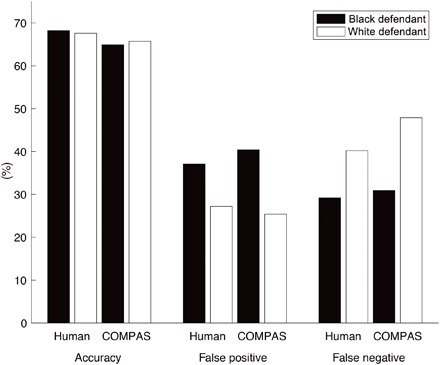
\includegraphics[width=8cm]{image1}
\caption{Die Ergebnisse der Studie [3], in der der COMPAS-Algorithmus mit zufällig gewählten Probanden bezüglich Aussagekraft der vorhergesehenen Rückfälligkeitswahrscheinlichkeit von Kriminellen verglichen wurde.\\ 
Die x-Achse beschreibt die Wahrscheinlichkeit für die auf der y-Achse beschriebenen Fälle. \\
Das erste paar Balken bezieht sich auf die Prognosen der Probanden, das zweite auf die Prognosen von COMPAS. \\
Die Farbe der Balken (schwarz oder weiß) entspricht der entsprechenden Ethnizität der Kriminellen.\\
Quelle: [3] }
\label{img1}
\end{figure}

\section{Aussicht auf den nächsten Blogeintrag}
% Genauso sind die Frage über die Aussagekräftigkeit der Studie aus Broward County, als auch ob genau COMPAS effizient ist, nicht unseres einziges Interesse zum diesem Algorithmen im Gericht.
% Im nächsten Beitrag untersuchen wir den Sozialen Aspekt davon und wir schauen uns, wie solcher Algorithm unsere Gesellschaft beeinflußen kann.
Im nächsten Beitrag in dieser Reihe zu Algorithmen im Gericht wird es darum gehen, die sozialen Gefüge, die durch Algorithmen wie COMPAS beeinflusst werden, zu betrachten, und zu analysieren, inwieweit es sich hier um ein sozioinformatisches System (nach Kienle und Kuhnau) handelt.

\section{Quellen}
\begin{itemize}
	\item{[1]}: Julia Angwin, Jeff Larson, Surya Mattu, Lauren Kirchner (ProPublica): \textit{“Machine Bias”}, 2016\\  
	         https://www.propublica.org/article/machine-bias-risk-assessments-in-criminal-sentencing (abgerufen am 19.03.2019)

	\item{ [2]}: Northpointe Inc.: \textit{"Practitioner’s Guide to COMPAS Core"}, 2015\\
	 https://assets.documentcloud.org/documents/2840784/Practitioner-s-Guide-to-COMPAS-Core.pdf (abgerufen am 19.03.2019)

	\item  {[3]} Julia Dressel, Hany Farid: \textit{"The accuracy, fairness, and limits of predicting recidivism"}, Publiziert 2018 in \textit{Science Advances Vol. 4, No. 1} \\ 
	       https://www.ncbi.nlm.nih.gov/pmc/articles/PMC5777393/  (abgerufen am 19.03.2019)
\end{itemize}





\printbibliography[title={Bibliography}] % Print the bibliography, section title in curly brackets

%----------------------------------------------------------------------------------------

\end{document}
